\documentclass{article}
\usepackage[UTF8]{ctex} 
\usepackage{amsmath}
\usepackage{bm}
\usepackage{amssymb}
\usepackage{geometry}
\usepackage{graphicx}
\usepackage{listings}
\usepackage{tikz}
\usepackage{amsthm}
\newtheorem{theorem}{定理}
\usetikzlibrary{calc}
\usetikzlibrary{shapes.multipart}
\usetikzlibrary{arrows.meta, positioning, shapes.geometric}
\usetikzlibrary{decorations.pathreplacing, fit}
\geometry{a4paper, margin=1.5cm}

\title{查找技术2}
\author{Tan Yiqing}
\date{\today}

\begin{document}
\maketitle
    
    \begin{figure}[h]
        \centering
        \includegraphics[width=0.65\textwidth]{D:/program/data_construction/firefly/微信图片_20251201171916_576_13.jpg}
    \end{figure}

\section{树表查找技术(续)}
\subsection{最小平衡二叉树的分类}
\indent 根据插入结点的位置不同,最小平衡二叉树的失衡类型可分为四种:\\
\begin{enumerate}
    \item LL型:在某结点的左子树的左子树上插入结点,导致该结点失衡。
    \item RR型:在某结点的右子树的右子树上插入结点,导致该结点失衡。
    \item LR型:在某结点的左子树的右子树上插入结点,导致该结点失衡。
    \item RL型:在某结点的右子树的左子树上插入结点,导致该结点失衡。
\end{enumerate}

\subsection{旋转调整方法}
\indent 为了恢复最小平衡二叉树的平衡性,需要对失衡的子树进行旋转调整。\\
\indent 先介绍一些调整方法:
\begin{enumerate}
    \item 右旋操作:假设以某结点为根
        \begin{enumerate}
            \item 将其左子结点->新的根
            \item 该结点->新根的右子结点
            \item 原左子结点的右子结点->该结点的左子结点
        \end{enumerate}
    \item 左旋操作:假设以某结点为根
        \begin{enumerate}
            \item 将其右子结点->新的根
            \item 该结点->新根的左子结点
            \item 原右子结点的左子结点->该结点的右子结点
        \end{enumerate}
\end{enumerate}

\indent 所以对于每一种失衡类型,旋转调整的方法如下:
\begin{enumerate}
    \item LL型失衡:对失衡结点进行右旋操作。
    \item RR型失衡:对失衡结点进行左旋操作。
    \item LR型失衡:先对失衡结点的\pmb{左子结点}进行左旋操作,然后对\pmb{失衡结点}进行右旋操作。
    \item RL型失衡:先对失衡结点的\pmb{右子结点}进行右旋操作,然后对\pmb{失衡结点}进行左旋操作。
\end{enumerate}

\textbf{1. LL型失衡(右旋)}

插入顺序:$30, 20, 10$,插入 $10$ 后 $30$ 失衡。

\begin{center}
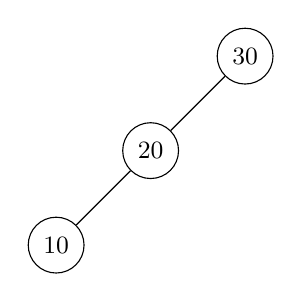
\begin{tikzpicture}[every node/.style={circle,draw,minimum size=7mm, font=\small}]
    \node (n30) at (0,0) {30};
    \node (n20) at (-1.2,-1.2) {20};
    \node (n10) at (-2.4,-2.4) {10};
    \draw (n30) -- (n20);
    \draw (n20) -- (n10);
\end{tikzpicture}
$\xrightarrow{\text{右旋}}$
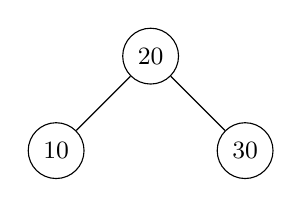
\begin{tikzpicture}[every node/.style={circle,draw,minimum size=7mm, font=\small}]
    \node (n20) at (0,0) {20};
    \node (n10) at (-1.2,-1.2) {10};
    \node (n30) at (1.2,-1.2) {30};
    \draw (n20) -- (n10);
    \draw (n20) -- (n30);
\end{tikzpicture}
\end{center}

\textbf{2. RR型失衡(左旋)}

插入顺序:$10, 20, 30$,插入 $30$ 后 $10$ 失衡。

\begin{center}
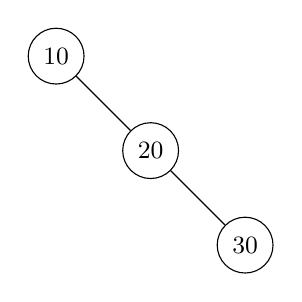
\begin{tikzpicture}[every node/.style={circle,draw,minimum size=7mm, font=\small}]
    \node (n10) at (0,0) {10};
    \node (n20) at (1.2,-1.2) {20};
    \node (n30) at (2.4,-2.4) {30};
    \draw (n10) -- (n20);
    \draw (n20) -- (n30);
\end{tikzpicture}
$\xrightarrow{\text{左旋}}$
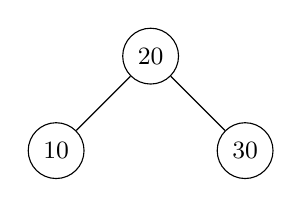
\begin{tikzpicture}[every node/.style={circle,draw,minimum size=7mm, font=\small}]
    \node (n20) at (0,0) {20};
    \node (n10) at (-1.2,-1.2) {10};
    \node (n30) at (1.2,-1.2) {30};
    \draw (n20) -- (n10);
    \draw (n20) -- (n30);
\end{tikzpicture}
\end{center}

\textbf{3. LR型失衡(先左旋再右旋)}

插入顺序:$30, 10, 20$,插入 $20$ 后 $30$ 失衡。

\begin{center}
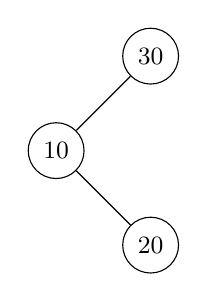
\begin{tikzpicture}[every node/.style={circle,draw,minimum size=7mm, font=\small}]
    \node (n30) at (0,0) {30};
    \node (n10) at (-1.2,-1.2) {10};
    \node (n20) at (0,-2.4) {20};
    \draw (n30) -- (n10);
    \draw (n10) -- (n20);
\end{tikzpicture}
$\xrightarrow{\text{左旋10}}$
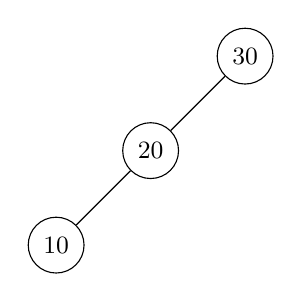
\begin{tikzpicture}[every node/.style={circle,draw,minimum size=7mm, font=\small}]
    \node (n30) at (0,0) {30};
    \node (n20) at (-1.2,-1.2) {20};
    \node (n10) at (-2.4,-2.4) {10};
    \draw (n30) -- (n20);
    \draw (n20) -- (n10);
\end{tikzpicture}
$\xrightarrow{\text{右旋30}}$
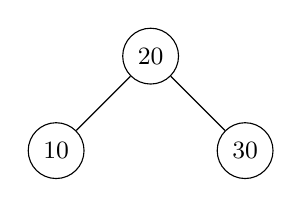
\begin{tikzpicture}[every node/.style={circle,draw,minimum size=7mm, font=\small}]
    \node (n20) at (0,0) {20};
    \node (n10) at (-1.2,-1.2) {10};
    \node (n30) at (1.2,-1.2) {30};
    \draw (n20) -- (n10);
    \draw (n20) -- (n30);
\end{tikzpicture}
\end{center}

\textbf{4. RL型失衡(先右旋再左旋)}

插入顺序:$10, 30, 20$,插入 $20$ 后 $10$ 失衡。

\begin{center}
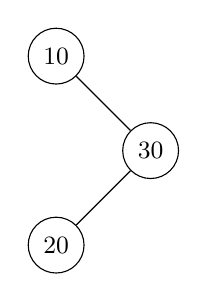
\begin{tikzpicture}[every node/.style={circle,draw,minimum size=7mm, font=\small}]
    \node (n10) at (0,0) {10};
    \node (n30) at (1.2,-1.2) {30};
    \node (n20) at (0,-2.4) {20};
    \draw (n10) -- (n30);
    \draw (n30) -- (n20);
\end{tikzpicture}
$\xrightarrow{\text{右旋30}}$
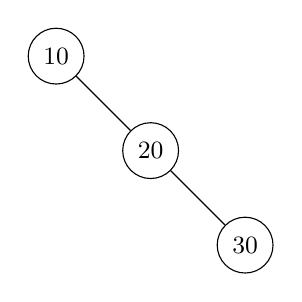
\begin{tikzpicture}[every node/.style={circle,draw,minimum size=7mm, font=\small}]
    \node (n10) at (0,0) {10};
    \node (n20) at (1.2,-1.2) {20};
    \node (n30) at (2.4,-2.4) {30};
    \draw (n10) -- (n20);
    \draw (n20) -- (n30);
\end{tikzpicture}
$\xrightarrow{\text{左旋10}}$
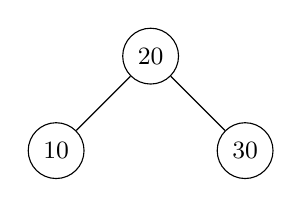
\begin{tikzpicture}[every node/.style={circle,draw,minimum size=7mm, font=\small}]
    \node (n20) at (0,0) {20};
    \node (n10) at (-1.2,-1.2) {10};
    \node (n30) at (1.2,-1.2) {30};
    \draw (n20) -- (n10);
    \draw (n20) -- (n30);
\end{tikzpicture}
\end{center}


\textbf{5. 复杂RL型失衡示例(包含子树移动)}

初始树包含结点:$50, 20, 80, 60, 90, 55$。插入结点 $70$ 后,根结点 $50$ 失衡。
失衡路径为 $50 \to 80 \to 60$,属于 RL 型。

\begin{center}
% Step 1: Imbalanced
\begin{tikzpicture}[every node/.style={circle,draw,minimum size=7mm, font=\small}, level distance=1.5cm]
    \node (n50) at (0,0) {50};
    \node (n20) at (-2,-1.5) {20};
    \node (n80) at (2,-1.5) {80};
    \node (n60) at (1,-3) {60};
    \node (n90) at (3,-3) {90};
    \node (n55) at (0.2,-4.5) {55};
    \node (n70) at (1.8,-4.5) {70};
    
    \draw (n50) -- (n20);
    \draw (n50) -- (n80);
    \draw (n80) -- (n60);
    \draw (n80) -- (n90);
    \draw (n60) -- (n55);
    \draw (n60) -- (n70);
    
    \node[draw=none] at (0, -5.5) {插入70,50失衡 (RL型)};
\end{tikzpicture}

\textbf{第一步:对失衡结点的右子结点(80)进行右旋}

% Step 2: Right Rotate 80
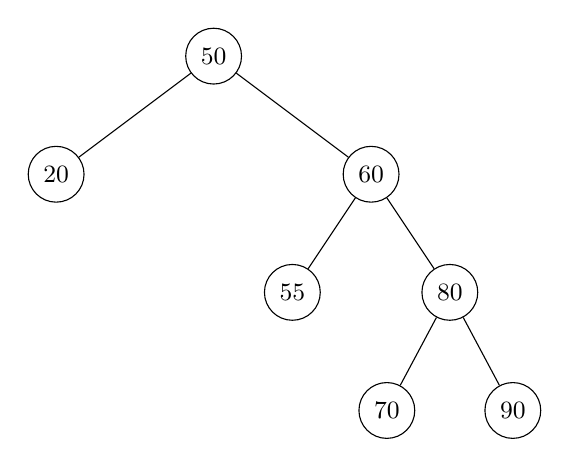
\begin{tikzpicture}[every node/.style={circle,draw,minimum size=7mm, font=\small}]
    \node (n50) at (0,0) {50};
    \node (n20) at (-2,-1.5) {20};
    \node (n60) at (2,-1.5) {60};
    \node (n55) at (1,-3) {55};
    \node (n80) at (3,-3) {80};
    \node (n70) at (2.2,-4.5) {70};
    \node (n90) at (3.8,-4.5) {90};

    \draw (n50) -- (n20);
    \draw (n50) -- (n60);
    \draw (n60) -- (n55);
    \draw (n60) -- (n80);
    \draw (n80) -- (n70);
    \draw (n80) -- (n90);
\end{tikzpicture}

\textbf{第二步:对失衡结点(50)进行左旋}

% Step 3: Left Rotate 50
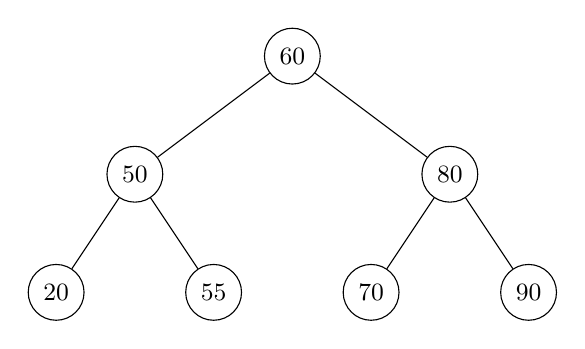
\begin{tikzpicture}[every node/.style={circle,draw,minimum size=7mm, font=\small}]
    \node (n60) at (0,0) {60};
    \node (n50) at (-2,-1.5) {50};
    \node (n80) at (2,-1.5) {80};
    \node (n20) at (-3,-3) {20};
    \node (n55) at (-1,-3) {55};
    \node (n70) at (1,-3) {70};
    \node (n90) at (3,-3) {90};

    \draw (n60) -- (n50);
    \draw (n60) -- (n80);
    \draw (n50) -- (n20);
    \draw (n50) -- (n55);
    \draw (n80) -- (n70);
    \draw (n80) -- (n90);
\end{tikzpicture}
\end{center}



\subsection{构造平衡二叉树}
\subsubsection{基本思想}
\indent 构造平衡二叉树(AVL树)时,每插入一个结点,需保证整棵树的平衡性。其基本思想如下:
\begin{enumerate}
    \item 插入新结点后,从插入点向上回溯,依次更新各祖先结点的平衡因子(BF)。若所有结点的平衡因子绝对值都不超过1,则树仍然平衡,无需调整。
    \item 若某个祖先结点的平衡因子绝对值超过1,说明树已失衡。此时,找到距离插入点最近的、平衡因子绝对值大于1的结点(即“最小不平衡子树”的根结点)。
    \item 根据新插入结点与该根结点之间的关系,判断属于哪种失衡类型(LL、RR、LR、RL),并进行相应的旋转调整(单旋或双旋),使该子树恢复平衡,从而整棵树重新成为平衡二叉树。
\end{enumerate}

\subsubsection{构造示例}
设有关键码序列 $\{5, 4, 2, 8, 6, 9\}$,构造平衡二叉树的过程如下:

\textbf{1. 插入 5, 4, 2 (LL型失衡)}

插入 2 后,结点 5 失衡 (LL型),需对 5 进行右旋。

\begin{center}
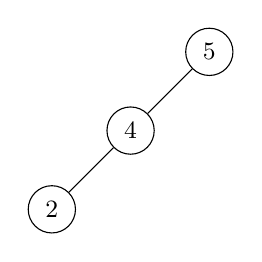
\begin{tikzpicture}[every node/.style={circle,draw,minimum size=6mm, font=\small}, level distance=1.2cm, sibling distance=1.2cm]
    \node (n5) at (0,0) {5};
    \node (n4) at (-1,-1) {4};
    \node (n2) at (-2,-2) {2};
    \draw (n5) -- (n4);
    \draw (n4) -- (n2);
\end{tikzpicture}
$\xrightarrow{\text{右旋5}}$
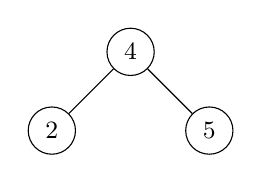
\begin{tikzpicture}[every node/.style={circle,draw,minimum size=6mm, font=\small}, level distance=1.2cm, sibling distance=1.2cm]
    \node (n4) at (0,0) {4};
    \node (n2) at (-1,-1) {2};
    \node (n5) at (1,-1) {5};
    \draw (n4) -- (n2);
    \draw (n4) -- (n5);
\end{tikzpicture}
\end{center}

\textbf{2. 插入 8 (平衡)}

\begin{center}
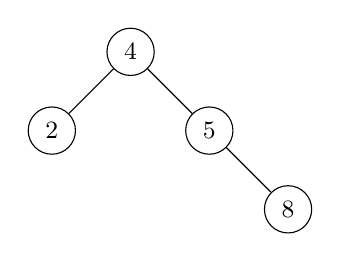
\begin{tikzpicture}[every node/.style={circle,draw,minimum size=6mm, font=\small}, level distance=1.2cm, sibling distance=1.2cm]
    \node (n4) at (0,0) {4};
    \node (n2) at (-1,-1) {2};
    \node (n5) at (1,-1) {5};
    \node (n8) at (2,-2) {8};
    \draw (n4) -- (n2);
    \draw (n4) -- (n5);
    \draw (n5) -- (n8);
\end{tikzpicture}
\end{center}

\textbf{3. 插入 6 (RL型失衡)}

插入 6 后,结点 5 失衡 (RL型:5右子树的左子树插入)。需先对 8 右旋,再对 5 左旋。

\begin{center}
\begin{tikzpicture}[every node/.style={circle,draw,minimum size=6mm, font=\small}, level distance=1.2cm, sibling distance=1.2cm]
    \node (n4) at (0,0) {4};
    \node (n2) at (-1.5,-1) {2};
    \node (n5) at (1.5,-1) {5};
    \node (n8) at (2.5,-2) {8};
    \node (n6) at (1.5,-3) {6};
    \draw (n4) -- (n2);
    \draw (n4) -- (n5);
    \draw (n5) -- (n8);
    \draw (n8) -- (n6);
    \node[draw=none] at (0,-3.5) {插入6,5失衡};
\end{tikzpicture}
$\xrightarrow{\text{调整后}}$
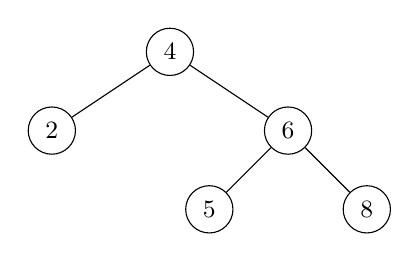
\begin{tikzpicture}[every node/.style={circle,draw,minimum size=6mm, font=\small}, level distance=1.2cm, sibling distance=1.2cm]
    \node (n4) at (0,0) {4};
    \node (n2) at (-1.5,-1) {2};
    \node (n6) at (1.5,-1) {6};
    \node (n5) at (0.5,-2) {5};
    \node (n8) at (2.5,-2) {8};
    \draw (n4) -- (n2);
    \draw (n4) -- (n6);
    \draw (n6) -- (n5);
    \draw (n6) -- (n8);
\end{tikzpicture}
\end{center}

\textbf{4. 插入 9 (RR型失衡)}

插入 9 后,根结点 4 失衡 (RR型:4右子树的右子树插入)。需对 4 进行左旋。

\begin{center}
\begin{tikzpicture}[every node/.style={circle,draw,minimum size=6mm, font=\small}, level distance=1.2cm, sibling distance=1.2cm]
    \node (n4) at (0,0) {4};
    \node (n2) at (-2,-1) {2};
    \node (n6) at (2,-1) {6};
    \node (n5) at (1,-2) {5};
    \node (n8) at (3,-2) {8};
    \node (n9) at (4,-3) {9};
    \draw (n4) -- (n2);
    \draw (n4) -- (n6);
    \draw (n6) -- (n5);
    \draw (n6) -- (n8);
    \draw (n8) -- (n9);
    \node[draw=none] at (0,-3.5) {插入9,4失衡};
\end{tikzpicture}
$\xrightarrow{\text{左旋4}}$
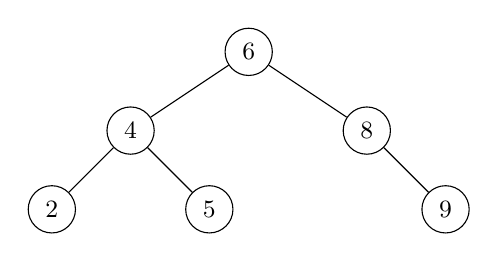
\begin{tikzpicture}[every node/.style={circle,draw,minimum size=6mm, font=\small}, level distance=1.2cm, sibling distance=1.2cm]
    \node (n6) at (0,0) {6};
    \node (n4) at (-1.5,-1) {4};
    \node (n8) at (1.5,-1) {8};
    \node (n2) at (-2.5,-2) {2};
    \node (n5) at (-0.5,-2) {5};
    \node (n9) at (2.5,-2) {9};
    \draw (n6) -- (n4);
    \draw (n6) -- (n8);
    \draw (n4) -- (n2);
    \draw (n4) -- (n5);
    \draw (n8) -- (n9);
    \end{tikzpicture}
    \end{center}


\section{散列表的查找技术}
基本思想:不用比较,在存储位置和关键码之间建立一个确定的对应关系,
通过关键码直接确定存储位置
\subsection{散列与其相关定义}
\begin{enumerate}
    \item 散列的基本思想:在记录的存储地址和它的关键码之间建立一个确定的对应关系。不经过比较,一次读取就能得到所查元素。
    \item 散列表:采用散列技术将记录存储在一块连续的存储空间中,这块连续的存储空间称为散列表。
    \item 散列函数:将关键码映射为散列表中适当存储位置的函数。
    \item 散列地址:由散列函数所得的存储地址。
    \item 冲突:对于两个不同关键码$k_i≠k_j$,有$H(k_i)=H(k_j)$,
    即两个不同的记录需要存放在同一个存储位置,$k_i$和$k_j$相对于$H$称做同义词。
\end{enumerate}

    \begin{figure}[h]
    \centering
    \begin{minipage}[t]{0.40\textwidth}
        \centering
        \includegraphics[width=\textwidth]{D:/program/data_construction/L7/理论/查找技术2/20251208175600.png}
    \end{minipage}
    \hfill
    \begin{minipage}[t]{0.40\textwidth}
        \centering
        \includegraphics[width=\textwidth]{D:/program/data_construction/L7/理论/查找技术2/搜狗截图20251208175647.png}
    \end{minipage}
\end{figure}

\subsection{散列技术的特点}
\begin{enumerate}
    \item 散列既是一种查找技术,也是一种存储技术。
    \begin{enumerate}
        \item 但只是通过记录的关键码定位该记录,没有完整地表达记录之间的逻辑关系。
        \item 所以,散列主要是面向查找的存储结构。
    \end{enumerate}
    \item 缺点:
    \begin{enumerate}
        \item 散列技术一般不适用于允许多个记录有同样关键码的情况。在散列表中,不可能找到最大或最小关键码的记录。
        \item 散列方法也不适用于范围查找。在散列表中,不可能找到在某一范围内的记录。
    \end{enumerate}
    \item 优点:速度快,适合回答“如果有的话,哪个记录的关键码等于待查值。”
    \item 散列技术的关键问题:
    \begin{enumerate}
        \item 如何设计一个简单、均匀、存储利用率高的散列函数。
        \item 如何采取合适的处理冲突方法来解决冲突。
    \end{enumerate}
\end{enumerate}

\subsection{散列函数的设计}
\indent 设计原则:计算简单,函数值(即散列地址)分布均匀。
\subsubsection{直接定址法}
散列函数是关键码的线性函数,即:
\[
    H(key) = a \ast  key + b
\]
其中a和b为常数,key为关键码。
\paragraph{举例:} 关键码集合为{10, 30, 50, 70, 80, 90},选取的散列函数为$H(key)=key/10$,则散列表为:
\begin{center}
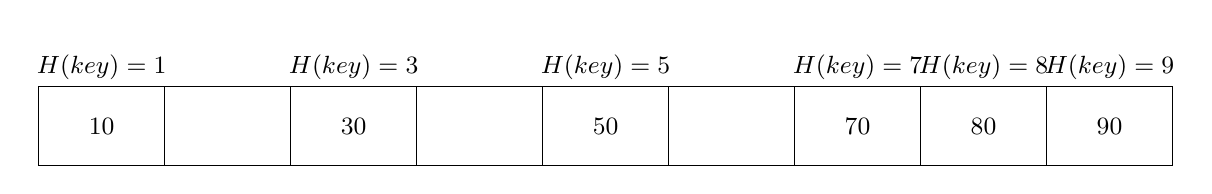
\begin{tikzpicture}[every node/.style={rectangle,draw,minimum width=1.6cm,minimum height=1cm, font=\small}]
    % 画9个连续框框
    \foreach \i in {1,...,9} {
        \draw (\i*1.6-1.6,0) rectangle (\i*1.6,1);
    }
    % 填关键码
    \node at (0.8,0.5) {10};
    \node at (3*1.6-0.8,0.5) {30};
    \node at (5*1.6-0.8,0.5) {50};
    \node at (7*1.6-0.8,0.5) {70};
    \node at (8*1.6-0.8,0.5) {80};
    \node at (9*1.6-0.8,0.5) {90};
    % 上方标注H(key)
    \foreach \i/\k in {1/10,3/30,5/50,7/70,8/80,9/90} {
        \node[draw=none] at (\i*1.6-0.8,1.25) {$H(key)=\i$};
    }
\end{tikzpicture}
\end{center}

\paragraph{使用情况} 事先知道关键码,关键码集合不是很大且连续性较好。

\subsubsection{除留余数法}
散列函数为:
\[
    H(key) = key \mod p
\]
$p$一般取为素数(或不包含小于20质因子的合数),且接近散列表长度m,这样可以产生较少的\pmb{冲突}。
\paragraph{举例:}自己根据上面例子想象一下。
\paragraph{使用情况:}最简单、最常用的构造散列函数的方法,不要求事先知道关键码的分布。

\subsubsection{数学分析法}
根据关键码在各个位上的分布情况,选取分布比较均匀的若干位组成散列地址。
\paragraph{举例:}关键码为8位十进制数,可选取其第2、4、6位组成散列地址(最好没有重复数字)。
\paragraph{使用情况:}能预先估计出全部关键码的每一位上各种数字出现的频度,不同的关键码集合需要重新分析。

\subsubsection{平方取中法}
对关键码平方后,按散列表大小,取中间的若干位作为散列地址(平方后截取)。
\paragraph{举例:}散列地址为2位,则关键码1234的散列地址为:$$H(1234) = 1234^2 = 1522756 \Rightarrow H(1234) = 27$$
\paragraph{使用情况:}关键码的位数比较均匀分布时事先不知道关键码的分布且关键码的位数不是很大。

\subsubsection{折叠法}
将关键码从左到右分割成位数相等的几部分,将这几部分叠加求和,取后几位作为散列地址。
\paragraph{举例:}关键码为12345678,分割成1234和5678两部分,求和得到6912,取后两位作为散列地址,即12。
\paragraph{使用情况:}关键码位数很多,事先不知道关键码的分布。

\subsection{冲突的处理}
\indent 开放定址法: 由关键码得到的散列地址一旦产生了冲突,就去寻找下一个空的散列地址,并将记录存入。
\indent 主要方法有线性探测法、二次探测法和随机探测法。
\subsubsection{线性探测法}
当发生冲突时,从冲突位置的下一个位置起,依次寻找空的散列地址。\\
\indent 对于键值$key$,设$H(key)=d$,闭散列表的长度为$m$,则发生冲突时,寻找下一个散列地址的公式为:
\[
    H_i = (H(key) + d_i) \mod m, \quad d_i = 1, 2, \ldots, m-1
\]
用开放定址法处理冲突得到的散列表叫\pmb{闭散列表}。

\paragraph{举例:} 关键码集合为 $\{47, 7, 29, 11, 16, 92, 22, 8, 3\}$,散列表表长为 $11$,散列函数为 $H(key)=key \bmod 11$,用线性探测法处理冲突,则散列表为:
\begin{center}
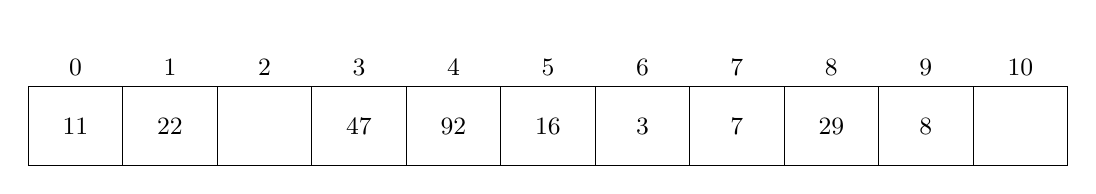
\begin{tikzpicture}[every node/.style={rectangle,draw,minimum width=1.2cm,minimum height=1cm, font=\small}]
    % 画11个连续框框
    \foreach \i in {0,...,10} {
        \draw (\i*1.2,0) rectangle (\i*1.2+1.2,1);
    }
    % 填关键码
    \node at (0.6,0.5) {11};   
    \node at (1.8,0.5) {22};  
       
    \node at (4.2,0.5) {47};   
    \node at (5.4,0.5) {92};   
    \node at (6.6,0.5) {16};   
    \node at (7.8,0.5) {3};  
    \node at (9.0,0.5) {7};    
    \node at (10.2,0.5) {29};
    \node at (11.4,0.5) {8};

    % 上方标注槽号
    \foreach \i in {0,...,10} {
        \node[draw=none] at (\i*1.2+0.6,1.25) {\i};
    }
\end{tikzpicture}
\end{center}
\noindent 注意:线性探测法容易产生\pmb{堆积},
即:在处理冲突的过程中出现的非同义词之间对同一个散列地址争夺的现象。

\paragraph{伪代码:}
\begin{enumerate}
    \item 计算散列地址j;
    \item 若ht[j]等于k,则查找成功,返回记录在散列表中的下标;否则执行第3步;
    \item 若ht[j]为空或整个散列表探测一遍,则查找失败,转4;否则,j指向下一单元,转2;
    \item 若整个散列表探测一遍,则表满,抛出溢出异常;否则,将待查值插入;
\end{enumerate} 

\subsubsection{二次探测法}
当发生冲突时,寻找下一个散列地址的公式为:
\[
    H_i = (H(key) + d_i) \bmod m \\
    \left( d_i = 1^2, -1^2, 2^2, -2^2, \ldots, q^2, -q^2 \quad \text{且} \quad q \leq \frac{m}{2} \right)
\]

\paragraph{举例:} 关键码集合为 $\{47, 7, 29, 11, 16, 92, 22, 8, 3\}$,散列表表长为 $11$,散列函数为 $H(key)=key \bmod 11$,用线性探测法处理冲突,则散列表为:
\begin{center}
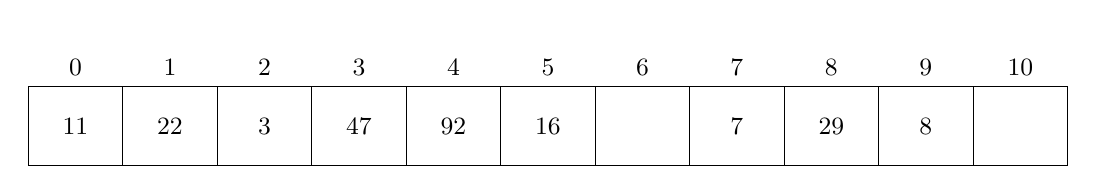
\begin{tikzpicture}[every node/.style={rectangle,draw,minimum width=1.2cm,minimum height=1cm, font=\small}]
    % 画11个连续框框
    \foreach \i in {0,...,10} {
        \draw (\i*1.2,0) rectangle (\i*1.2+1.2,1);
    }
    % 填关键码
    \node at (0.6,0.5) {11};   
    \node at (1.8,0.5) {22};  
    \node at (3.0,0.5) {3};
    \node at (4.2,0.5) {47};   
    \node at (5.4,0.5) {92};   
    \node at (6.6,0.5) {16};   
    \node at (7.8,0.5) {};  
    \node at (9.0,0.5) {7};    
    \node at (10.2,0.5) {29};
    \node at (11.4,0.5) {8};

    % 上方标注槽号
    \foreach \i in {0,...,10} {
        \node[draw=none] at (\i*1.2+0.6,1.25) {\i};
    }
\end{tikzpicture}
\end{center}

\subsubsection{随机探测法}
当发生冲突时,下一个散列地址的位移量是一个随机数列,即寻找下一个散列地址的公式为:
\[
    H_i = (H(key) + d_i) \bmod m
\]
其中 $d_i$ 是一个随机数列,$i=1,2,\ldots,m-1$。
随机的本质是伪随机,这里计算机产生随机是通过线性同余法:
\[
    \begin{cases}
        a_0 = d \\
        a_{i+1} = (b \ast a_i + c) \bmod m
    \end{cases}
\]
其中,$d$称为随机种子。当$b$、$c$和$m$的值确定后,给定一个随机种子,产生确定的随机数序列。

\subsubsection{拉链法}
将所有散列地址相同的记录,即所有同义词记录存储在一个单链表中(称为\pmb{同义词子表}),在散列表中存储的是所有同义词子表的头指针。
用拉链法处理冲突构造的散列表叫做\pmb{开散列表}。开散列表不会出现堆积现象。\\
\indent 设$n$个记录存储在长度为$m$的散列表中,则同义词子表的平均长度为$n / m$。

\paragraph{举例:} 关键码集合为 $\{47, 7, 29, 11, 16, 92, 22, 8, 3\}$,散列表表长为 $11$,散列函数为 $H(key)=key \bmod 11$,用拉链法,则散列表为:

\begin{figure}[h]
    \centering
    \includegraphics[width=0.3\textwidth]{D:/program/data_construction/L7/理论/查找技术2/搜狗截图20251208194546.png}
\end{figure}

\paragraph{伪代码:}
\begin{enumerate}
    \item 计算散列地址j;
    \item 在第j个同义词子表中顺序查找;
    \item 若查找成功,则返回结点的地址;
    否则,将待查记录插在第j个同义词子表的表头。
\end{enumerate}

\subsection{性能分析}
由于冲突的存在,产生冲突后的查找仍然是给定值与关键码进行比较的过程。
在查找过程中,关键码的比较次数取决于产生冲突的概率。影响冲突产生的因素有:
\begin{enumerate}
    \item 散列函数是否均匀;
    \item 处理冲突的方法;
    \item 散列表的装载因子。
\end{enumerate}
记:
\[
    \alpha = \frac{n}{m}
\]
为散列表的\pmb{装载因子},其中$n$为散列表中填入的记录数,$m$为散列表的长度。
\begin{figure}[h]
    \centering
    \includegraphics[width=0.6\textwidth]{D:/program/data_construction/L7/理论/查找技术2/图片1.png}
\end{figure}
散列表的平均查找长度是装填因子$\alpha$的函数,散列表在空间换时间。

\subsection{开散列表与闭散列表的对比}


\begin{center}
\begin{tabular}{|c|p{5cm}|p{5cm}|}
    \hline
    \textbf{对比项} & \textbf{开散列表(拉链法)} & \textbf{闭散列表(开放定址法)} \\
    \hline
    冲突处理方式 & 同义词用链表存储在同一槽 & 冲突时在表内寻找下一个空槽 \\
    \hline
    估计容量 & 不需要(链表可扩展) & 需要(表满即不能插入) \\
    \hline
    查找效率 & 效率高,受链表长度影响,装载因子大时效率下降较慢 & 效率低,装载因子大时查找效率急剧下降 \\
    \hline
    删除操作 & 简单,直接删除链表结点 & 复杂,需特殊标记或重排 \\
    \hline
    结构开销 & 有,需要额外存储指针 & 无 \\
    \hline
    适用场景 & 适合经常插入、删除的场景 & 适合查找多、删除少的场景 \\
    \hline
    是否易产生堆积 & 不产生堆积 & 易产生堆积 \\
    \hline
\end{tabular}
\end{center}

\end{document}